\documentclass{article}
\usepackage{amsmath}
\usepackage{url}
\usepackage{graphicx}
\usepackage{subcaption}
\title{Contextual BO experiment}
\author{Feng Zhao}

\begin{document}
\maketitle
\section{Experiment 1}
Using Contextual BO to find the maximal value of $f(x,y)$ for given $y$.
\begin{equation}
    f(x,y) = \cos(2 x) \cos(y) + \sin(x)
\end{equation}
Choosing $x,y \in [0,6]$. Our goal is to provide a surrogate model of $z=g(y)=\arg\max_{x} f(x,y)$.
The exact solution is non-continuous, which means that it is very hard to estimate $z=g(y)$ at the
non-continuous points.
\begin{figure}[!ht]
    \centering
    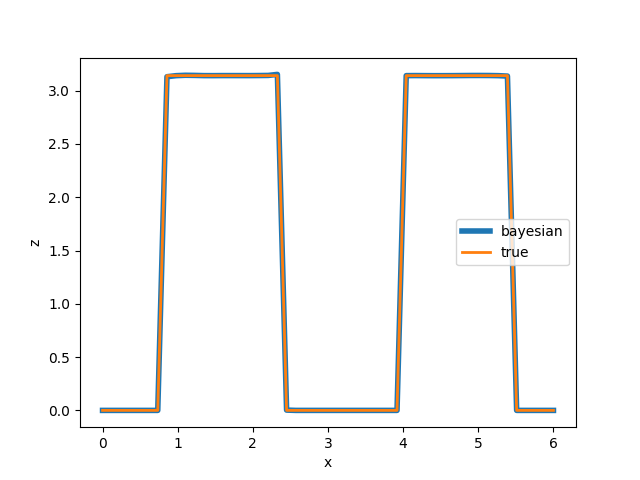
\includegraphics[width=6cm]{cbo_1.png}
\end{figure}
\end{document}


